\chapter{Arquitetura de bancos de dados}
\label{arquitetura-bd}

A arquitetura básica de um banco de dados relacional é composta de um cliente e de um servidor, como pode ser visualizado na figura \ref{fig:client-server}. O cliente possui poucas funcionalidades próprias, sendo utilizado apenas como interface entre o servidor e o usuário. O servidor, por outro lado, é responsável por todo o processamento das consultas. Essa separação entre cliente e servidor favorece a independência de dados, onde o cliente não precisa saber como os dados são fisicamente armazenados, simplificando o desenvolvimento de novas aplicações \cite[p. 30]{Bell:2012}.

A comunicação entre aplicações cliente e servidor geralmente é feita através de uma conexão de rede, mas também pode ser realizada por estruturas internas do sistema operacional (\emph{sockets}, \emph{pipes}, etc.) ou integrando-se o banco de dados à aplicação (\gls{sgbd} embarcado). Qualquer que seja o meio de comunicação utilizado, o cliente envia consultas para o servidor, que a processa e retorna o resultado para o cliente.

\begin{figure}[H]
  \centering
  \caption{Modelo de comunicação cliente/servidor em bancos de dados relacionais.}
  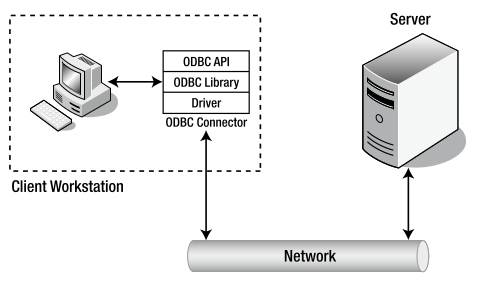
\includegraphics[width=.65\textwidth]{images/client-server-model.png}
  \fonte{\citet[p. 28]{Bell:2012}}
  \label{fig:client-server}
\end{figure}

Nas seções seguintes é descrita a estrutura interna de cada um dos elementos que compõem a arquitetura de um banco de dados relacional. A seção \ref{modelo-relacional} descreve o modelo relacional proposto por E. F. Codd, no qual os \glspl{sgbd} relacionais são baseados. Na seção \ref{aplicacao-cliente} é abordado o funcionamento da aplicação cliente, bem como a forma de apresentação das consultas e dos resultados. A seção \ref{interface-comunicacao} descreve como é feita a comunicação entre as aplicações cliente e servidor, e as estruturas utilizadas para esta finalidade. Por fim, a seção \ref{processamento-consultas} expõe as etapas de processamento das consultas no servidor, incluindo os estágios de análise léxica e sintática, a geração do plano de execução e a efetiva realização da operação requisitada pelo cliente.



\section{Modelo relacional}
\label{modelo-relacional}

O modelo de dados relacional proposto inicialmente por E. F. Codd em 1970 define o conceito de um método de armazenamento de dados que pode ser acessado e manipulado utilizando uma linguagem de consulta \cite[p. 25]{Bell:2012}. Devido à sua simplicidade e bom embasamento teórico e matemático, o modelo tornou-se o mais utilizado para armazenamento de dados estruturados \cite{Lightstone:2007}.

No modelo relacional, os dados são representados como informações (atributos) sobre uma determinada entidade. Um registro ou tupla contém os valores para os atributos de uma entidade. As tabelas são um conjunto de registros que possuem os mesmos atributos, e podem ser relacionadas a outras tabelas utilizando-se restrições (\emph{constraints}).

Não existe uma linguagem de consulta padrão definida pelo modelo relacional. Contudo, muitas aplicações optaram por implementar a \gls{sql}, uma linguagem de consulta que se assemelha com linguagem natural. Atualmente, a \gls{sql} é o padrão do mercado, sendo suportada pelos \glspl{sgbd} mais conhecidos e utilizados \cite[p. 26]{Bell:2012}.



\section{Aplicação cliente}
\label{aplicacao-cliente}

Uma aplicação cliente pode ser qualquer \emph{software} que se comunique com o \gls{sgbd} para manipular os dados de alguma forma. Essa definição inclui tanto aplicações desenvolvidas para serem utilizadas por usuários finais quanto aplicações de gerenciamento e modelagem do banco de dados. Qualquer \emph{software} cliente envia comandos para o servidor utilizando, geralmente, a linguagem \gls{sql}, recebe a resposta e exibe para o usuário.

Os comandos \gls{sql} podem ser divididos em duas categorias principais: \gls{ddl}, utilizada para criação das estruturas de armazenamento dos dados, como tabelas e índices, e a \gls{dml}, responsável pelas operações de manipulação dos dados armazenados, como criação de novos registros, modificação dos dados já existentes e recuperação dos dados salvos.

Cada comando \gls{sql} possui uma sintaxe própria e bem-definida. Todos possuem a especificação de uma ação, por exemplo criar uma tabela (CREATE TABLE) ou atualizar dados (UPDATE). Em seguida são informados demais parâmetros que afetam o tipo de estrutura que será criado ou os dados que serão atingidos.



\section{Interface de comunicação}
\label{interface-comunicacao}

Existem, de maneira geral, duas diferentes formas de comunicação entre uma aplicação cliente e o \gls{sgbd}. Em uma delas, o cliente e o servidor são processos separados, e a comunicação ocorre utilizando alguma interface de rede ou estruturas especiais oferecidas pelo sistema operacional, como \emph{pipes}, \emph{FIFOs} e \emph{sockets}. Esse meio de comunicação é o mais comum e é utilizado na maioria das aplicações modernas. Utilizam o conceito de envio de consultas \gls{sql} para o servidor e o retorno da resposta para o cliente utilizando um protocolo de comunicação padronizado, geralmente o \gls{odbc} ou uma de suas variantes, como o \gls{jdbc}. Estes protocolos definem o formato das mensagens enviados entre cliente e servidor, além de promover uma forma de acesso padrão para diferentes \glspl{sgbd}.

Outra forma de comunicação é o uso de um \gls{sgbd} embarcado. Dessa forma, a aplicação cliente utiliza funções disponibilizadas em uma \gls{api} fornecida pelo banco de dados para acessar diretamente os arquivos de armazenamento dos dados. O exemplo de banco de dados mais conhecido que oferece essa funcionalidade é o SQLite\footnote{SQLite: http://sqlite.org/}, porém outros bancos de dados também oferecem suporte a essa opção \cite[p. 195]{Bell:2012}. Mesmo nessa modalidade, as consultas ainda são escritas em \gls{sql} ou em outra linguagem suportada.



\section{Processamento de consultas}
\label{processamento-consultas}

Em bancos de dados que seguem o modelo cliente/servidor, o processamento das consultas é feito de forma sequencial no servidor e separado em várias etapas. Cada etapa é responsável por realizar alguma operação ou transformação sobre a consulta e gerar uma saída, que será utilizada na próxima etapa. Uma visão geral do processo de execução das consultas é exibido na figura \ref{fig:etapas-execucao-consulta}.

\begin{figure}[ht]
  \centering
  \caption{Etapas do processamento de consultas em um SGBD relacional.}
  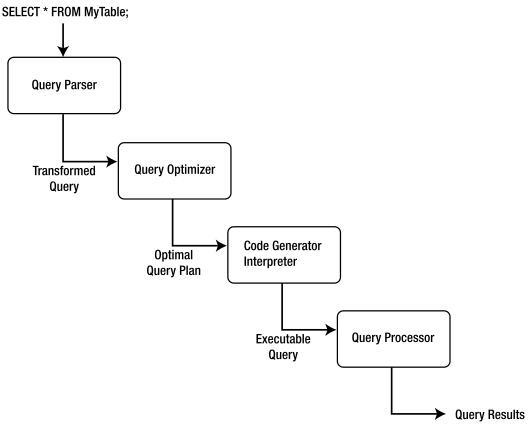
\includegraphics[width=.8\textwidth]{images/etapas-execucao-consulta.png}
  \fonte{\citet[p. 33]{Bell:2012}}
  \label{fig:etapas-execucao-consulta}
\end{figure}

A primeira tarefa executada quando uma nova consulta é recebida pelo servidor é a análise e interpretação do seu significado (\emph{Query Parser}). Considerando uma consulta escrita em \gls{sql}, é necessário identificar os atributos e tabelas que o cliente deseja acessar, e quais as condições definidas para restringir os registros que devem ser retornados. Todas essas informações devem ser extraídas da consulta recebida e convertidas para uma estrutura com a qual o \gls{sgbd} possa trabalhar nas etapas seguintes.

A consulta é convertida para uma estrutura em árvore identificando os componentes da lógica relacional, isto é, quais atributos devem ser retornados (projeção), quais junções entre tabelas devem ser realizadas, quais critérios de seleção devem ser aplicados e, caso indicado na consulta, as funções de agregação e ordenação que devem ser aplicadas. Todas essas informações formam a estrutura gerada pela etapa de análise da consulta.

Após a criação da árvore de consulta, na etapa seguinte (\emph{Query Optimizer}) são identificadas as possíveis abordagens para acesso aos dados e realização da junção entre tabelas. Essa tarefa é executada pelo otimizador, que é responsável por montar um plano de execução otimizado para a consulta a ser efetuada.

Existem quatro principais meios de otimização de consultas que são utilizados em \glspl{sgbd} relacionais \cite{Bell:2012}. 1) A otimização baseada em custo gera vários planos de execução equivalentes e então escolhe o que possui o menor custo, baseado em estatísticas coletadas em consultas anteriores. 2) A otimização heurística implementa algumas boas práticas para execução da consulta, utilizando algumas regras para eliminar os casos que provavelmente apresentariam um desempenho ruim e sugerindo opções que possivelmente apresentem alguma melhoria na performance.

A combinação dos métodos de otimização baseada em custo e heurísticas resulta na (3) otimização paramétrica, visando reduzir a quantidade de planos de execução a serem avaliados, através do uso de funções heurísticas para ignorar os piores planos. Uma quarta alternativa, que ainda não é implementada em \glspl{sgbd} comerciais, é a (4) otimização semântica, que ainda está em pesquisa, cujo objetivo é que o otimizador tenha conhecimento do esquema do banco de dados e das restrições existentes, simplificando partes da consulta automaticamente.

A saída do otimizador é o plano de execução que foi escolhido de acordo com os parâmetros de performance como sendo o mais otimizado. Na etapa seguinte (\emph{Code Generator Interpreter}), o plano é convertido em um algoritmo para acessar as estruturas físicas de armazenamento dos dados, como os índices e as tabelas. A etapa de execução da consulta (\emph{Query Processor}) pode ser implementada utilizando duas estratégias: iterativa e interpretativa.

A estratégia interpretativa consiste em transformar o plano de execução em uma sequência de chamada de funções pré-compiladas. As funções utilizadas são implementadas de forma genérica e executam tarefas básicas do processamento da consulta, não sendo otimizadas para nenhum caso específico. É a mais utilizada em sistemas de bancos de dados relacionais \cite[p. 35]{Bell:2012}.

Na estratégia iterativa, o \gls{sgbd} implementa funções para operações discretas (junção, projeção, etc.). O processamento da consulta consiste na transformação do plano de execução em um programa que utiliza essas funções disponibilizadas pelo banco de dados e subsequente compilação do mesmo em um arquivo binário executável.

Para recuperar as informações solicitadas, o \gls{sgbd} precisa definir como será feito o acesso aos dados no disco. A estrutura mais utilizada nos bancos de dados modernos são arquivos, acessados por meio do sistema de arquivos do sistema operacional. Um motor de armazenamento (\emph{storage engine}) estabelece a estrutura e forma de acesso aos arquivos, tendo como principal objetivo minimizar os custos de operações de entrada e saída (E/S). Com essa finalidade, alguns dos métodos mais empregados são o uso de estruturas que permitam acessar apenas as informações relevantes do disco, um mecanismo de \emph{cache} ou \emph{buffer} para aprimorar o tempo de leitura dos dados, e o uso de índices para auxiliar a obter os registros desejados.
